\documentclass{article}%
\usepackage[T1]{fontenc}%
\usepackage[utf8]{inputenc}%
\usepackage{lmodern}%
\usepackage{textcomp}%
\usepackage{lastpage}%
\usepackage{authblk}%
\usepackage{graphicx}%
%
\title{The effect of transforming growth factor \_1 on the crosstalk between autophagy and apoptosis in the annulus fibrosus cells under serum deprivation}%
\author{George Shea}%
\affil{Department of Pediatrics and Molecular and Cellular Oncology, The University of Texas M. D. Anderson Cancer Center, Houston, TX, USA}%
\date{01{-}01{-}2014}%
%
\begin{document}%
\normalsize%
\maketitle%
\section{Abstract}%
\label{sec:Abstract}%
Transmyeloma is another type of cancer which has been linked to the development of lupus nephritis, an inflammation of the liver (ciliary dysfunction) that causes a buildup of swelling and scarring in the liver, and an an infection of the livers organ.\newline%
This may be a common condition among rheumatoid arthritis (RA) patients, but according to a recent study, researchers at The Scripps Research Institute have discovered that increased serum anti{-}ribosomal{-}PBA antibodies may also turn the lehter an autoimmune pemphigoid disorder (LAP) into lupus nephritis.\newline%
The study, published in the journal Anti{-}Serum Antibiotics and Immunology, is based on an analysis of blood samples of 66 lupus nephritis patients (40 percent who developed LAP and had a chronic liver disease), identified as having lupus before initiating treatment and study and included immune{-}oncology researchers from The Scripps Research Institute (TSRI) who provide unique insight into the mechanisms involved in lupus nephritis.\newline%
In this early, important study, we identified lupus nephritis, an infection of the liver in which secretion of inflammatory antigens leads to scarring of liver (C{-}NAT), which we think is a possible mechanism driving lupus nephritis, said Jeremy Levin, Ph.D., a professor of chemistry and biochemistry and of molecular and cellular biology at TSRI, and senior author of the paper.\newline%
Lupus nephritis can be detected in the liver via blood, throat or nasal samples.

%
\subsection{Image Analysis}%
\label{subsec:ImageAnalysis}%


\begin{figure}[h!]%
\centering%
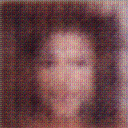
\includegraphics[width=150px]{500_fake_images/samples_5_232.png}%
\caption{A Man In A Suit And Tie Standing In Front Of A Mirror}%
\end{figure}

%
\end{document}